\documentclass[12pt, twoside]{article}
\usepackage[letterpaper, margin=1in, headsep=0.5in]{geometry}
\usepackage[english]{babel}
\usepackage[utf8]{inputenc}
\usepackage{amsmath}
\usepackage{amsfonts}
\usepackage{amssymb}
\usepackage{tikz}
\usetikzlibrary{quotes, angles}
\usepackage{graphicx}
\usepackage{enumitem}
\usepackage{multicol}
\usepackage{hyperref}

\newif\ifmeta
\metatrue %print standards and topics tags

\title{IB Mathematics}
\author{Chris Huson}
\date{March 2022}

\usepackage{fancyhdr}
\pagestyle{fancy}
\fancyhf{}
\renewcommand{\headrulewidth}{0pt} % disable the underline of the header
\raggedbottom


\fancyhead[LE]{\thepage}
\fancyhead[RO]{\thepage \\ Name: \hspace{4cm} \,\\}
\fancyhead[LO]{BECA / IB Math 5 Exponential functions \\* 7 March 2022}

\begin{document}
\subsubsection*{5.9 Prequiz: Exponential functions}
\emph{Round all currency amounts to the nearest hundredth.}
\begin{enumerate}
\item Isabella puts \$1,000 into an investment account with an annual interest rate of 4.00\%. Find the balance after one year. \vspace{1.5cm}

\item Louise invests \$8,750 in an account with an annual interest rate of 3.95\%. Find the balance after 4 years. \vspace{1.5cm}

\item William puts \$10,000 into an investment account with an annual interest rate of 5.75\%. Find the number of years required for the balance to reach \$14,789.81. \vspace{2cm}

\item A bond with a three year maturity and principal amount of \$20,000 compounds semi-annually with an annual interest rate of 4.25\%.
\begin{enumerate}[itemsep=0.5cm]
    \item How many compounding periods are there per year? \\[0.25cm]
    $k=$
    \item Find the final balance of principal and interest after three years.
\end{enumerate} \vspace{1.5cm}

\item Xi invested TWD 4000 (Taiwan dollars) in an account that pays 2.85\% interest per year compounded monthly. (show your working with a labeled sketch)
\begin{multicols}{2}
    \begin{enumerate}[itemsep=1cm]
        \item Find how much Xi had in the account after 3 years.
        \item Find the number of years until he had TWD 5000 in the account.
    \end{enumerate} \vspace{0.5cm}
    \begin{center}
    \begin{tikzpicture}
        \draw [thick, ->] (0,0)--(5,0);
        \draw [thick, ->] (0,0)--(0,6);
    \end{tikzpicture}
    \end{center}
\end{multicols}


\newpage
\item The graph shows the exponential function $\displaystyle FV=1,250 \times \left( 1+\frac{4.25}{100} \right)^t$ representing the balance of an investment account earning a fixed rate of interest over $t$ in years.
\begin{multicols}{2}
    \begin{enumerate}[itemsep=1cm]
        \item Write down the initial deposit in the account.
        \item Write down the annual interest rate.
        \item How much will the account hold at the end of ten years, to the nearest \$000?
        \item When will the balance be \$1,600?
    \end{enumerate}
    \begin{center}
    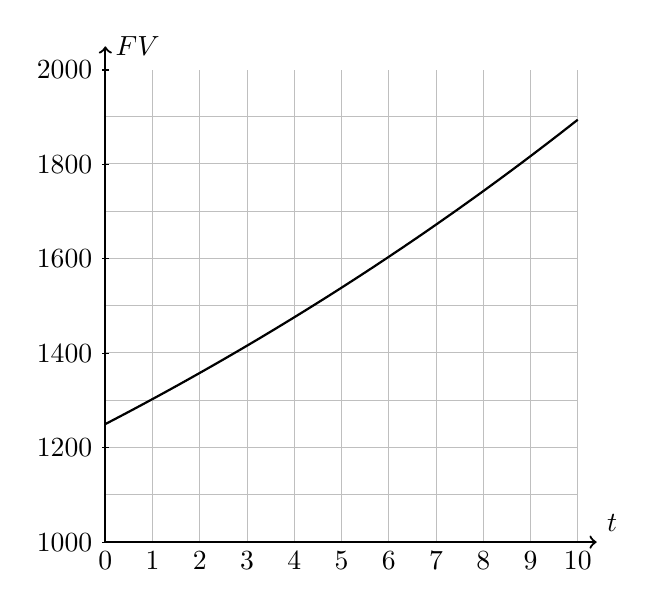
\begin{tikzpicture}[x=1cm, y=0.01cm, scale=0.6]
        \draw [thin, color=lightgray, xstep=1.0cm,ystep=1.0cm] (0,1000) grid (10,2000);
        \draw [thick, ->] (0,1000) -- (+10.4,1000) node [above right]{$t$};
        \draw [thick, ->] (0,1000) -- (0,2050) node [right]{$FV$};        \foreach \x in {0,1,...,10}
            \draw (\x cm,1000) -- (\x cm,1000) node[below] {$\x$};
        \foreach \y in {1000,1200,...,2000}
            \draw[shift={(0,\y)}] (2pt,0pt)--(-2pt,0pt) node[left]{$\y$};

        \draw [thick, smooth,domain=0.:10] plot(\x,{1250*(1.0425^\x)});
    \end{tikzpicture}
    \end{center}
    \end{multicols}

\item Radioactive elements decay over time, with one half of the atoms decaying over a fixed period of time, the ``half life.'' The half life of plutonium-238 is about 90 years. Use the formula $\displaystyle y=A \times \left( \frac{1}{2} \right)^{t/90}$. 
    \begin{enumerate}[itemsep=1.5cm]
        \item Find the percentage of plutonium that would remain after 1000 years.
        \item Find the number of years required for 99 percent of the plutonium to decay.
    \end{enumerate}

\item The spread of a farm disease can be modeled by the equation $\displaystyle y= 6 + e^x$, where $x$ is the time in days. 
    \begin{enumerate}[itemsep=1.5cm]
        \item Find the number of animals with the disease after six days.
        \item Find the number of days for 500 animals to be infected.
    \end{enumerate}
    
\item On the grid below draw the exponential function $\displaystyle f(t)=1700 \times \left( 1+0.095 \right)^t$ representing the growth of an investment over $t$ years.
\begin{multicols}{2}
    \begin{enumerate}[itemsep=1.2cm]
        \item Write down the initial value of the investment.
        \item Write down the annual interest rate.
        \item Find the value of the investment after ten years.\vspace{1cm}
        \item Find the number of years it takes the investment to double in value.
    \end{enumerate}
    \begin{center}
    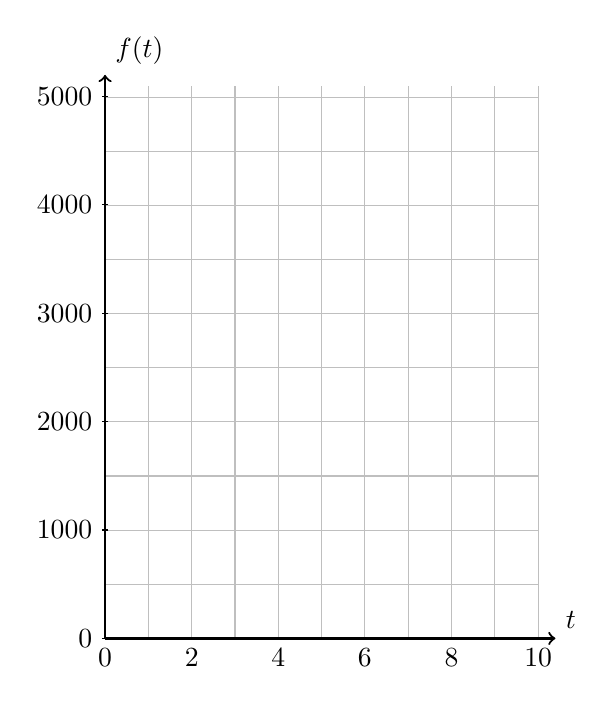
\begin{tikzpicture}[x=1cm, y=0.0025cm, scale=0.55]
        \draw [thin, color=lightgray,xstep=1.0cm,ystep=1.25cm](0,0) grid (10,5100);
        \draw [thick, ->] (0,0) -- (+10.4,0) node [above right]{$t$};
        \draw [thick, ->] (0,0) -- (0,5200) node [above right]{$f(t)$};        
        \foreach \x in {0,2,...,10}
            \draw (\x cm,0) -- (\x cm,0) node[below] {$\x$};
        \foreach \y in {0,1000,...,5000}
            \draw[shift={(0,\y)}] (2pt,0pt)--(-2pt,0pt) node[left]{$\y$};
        %\draw [thick, smooth,domain=0:10] plot(\x,{1700*(1.095^\x)});
    \end{tikzpicture}
    \end{center}
    \end{multicols}

\item A rabbit population doubles every 4 weeks. There are currently five rabbits in a restricted area. With $t$ representing time, in weeks, then the population of rabbits can be modeled by \[\displaystyle P(t)=A \times b^{t/4}\]
    %Alg2 Regents Jan2017
    \begin{enumerate}[itemsep=0.75cm]
        \item Write down the value of $A$
        \item Write down the value of $b$
        \item About how many rabbits will there be in 98 days? \vspace{2cm}
        \item After how many weeks will there be approximately 160 rabbits?
    \end{enumerate}

\item The temperature of a hot iron as it cools is modeled by the function 
    \[ T(x)=350e^{-0.035x}+18 \] where $T(x)$
    is the temperature in degrees Celsius and $x$ is the time in minutes.
    \begin{enumerate}[itemsep=1cm]
        \item Write down the initial temperature at time zero.
        \item Find the temperature after 20 minutes.
        \item When will the temperature of the iron reach 75 degrees Celsius?
        \item On the graph below, sketch the temperature of the iron, labeling the points above A, B, and C.
    \end{enumerate}
    \begin{center}
    \begin{tikzpicture}[xscale= 0.2, yscale=0.015]
        \draw [thick, ->] (0,0) -- (62,0) node [right] {$x$};
        \draw [thick, ->] (0,0) -- (0,550) node [right] {$T(x)$};
        \foreach \x in {0,10,20,30,40,50,60}
            \draw[shift={(\x,0)}] (0,10) -- (0,0) node[below]  {$\x$};
        \foreach \y in {0,100,200,300,400,500}
            \draw[shift={(0,\y)}] (0.5,0) -- (0,0) node[left]  {$\y$};
        %\draw [<-, ->] plot[domain= 0:60] (\x,{350*exp(-0.035*\x) +18});
        %\draw plot[domain=0:60] (\x, 75);
    \end{tikzpicture}
    \end{center}

\end{enumerate}
\end{document}
